The term \emph{business process modeling} is first introduced by S. Williams \cite{swill} where he argues that the techniques for modeling physical control systems could be applied to business processes \cite{tdj03}. However, it took until the 1990s for the term \emph{business process} to become popular \cite{Hook11}. 

At the time, companies started to think in terms of processes rather than functions and procedures \cite{wiki3}. Process thinking ensures the right development direction by analyzing the chain of events in an organization. Examples include the events occurring from purchase to supply or from receiving orders to sales.

%Unlike the traditional modeling tools, which focus on calculating time and costs, the modern modeling techniques consider the cross-functional activities. As a result of growing complexity and dependency between activities, 
%such cross-functionalities are significantly increasing in both size and importance \cite{wiki3}. 
 
A \emph{business process} is a set of related and structured activities, which serves a specific goal for a customer \cite{wiki3}. The de-facto standard in the field of business process modeling is the Business Process Model and Notation (BPMN). 

%BPMN is a graph based process definition language, which provides a graphical notation for specifying business processes. The main goal of BPMN to provide a standard common language between various business stakeholders including technical and business users \cite{whyformalbpmn}. As a result, BPMN aims at bridging the often occurring gap between business process design and implementation.
Business Process Model and Notation (BPMN) \cite{BPMN20}, previously referred to as Business Process Modeling Notation, is a graphical representation of business process models based on flowcharting techniques. The main goal of BPMN is to provide an understandable notation for both technical experts and business users. %It aims at bridging the communication gap between business stakeholders and technical experts.

%BPMN is able to model complex business processes using its diverse set of control structures, which range over sequencing, repetition, choice, concurrency, timeout, messaging, failure, transactions, etc. %It also provide notation for describing roles required to run each activity. 
%It has an expressive notation for defining events and associating triggers to them. Furthermore, it provides means to form reusable units out of a set of BPMN elements. 
%%

Similar to many modeling languages, it is possible for a BPMN model to contain errors. Syntactical errors are created by connecting the modeling elements in an invalid manner. %For example, an event that has two outgoing edges rather than one.
 In general, syntactical errors can be detected simply by parsing the model \cite{deadlockbpmn}. A number of BPMN designing tools such as Eclipse BPMN Modeler \cite{BPMN2modeler}, ARIS Express \cite{arisexpress}, and Yaoqiang \cite{Yaoqiang} can detect syntactical errors in models. 

However, a model may contain behavioral errors, which are more complicated to detect. For instance, a model may represent a process that is not \emph{sound}. A process is sound when every reachable state from an initial state has a way to reach a final state \cite{RPU+07}. A process may contain \emph{deadlock} or \emph{livelock}. Deadlocks occur when a process can reach a non-final state that it cannot leave. Livelocks happen when a process ends in one path, but some states are still active with no progress possible. Detecting behavioral errors requires investigating the runtime behavior of a process. An informal approach to finding cases of deadlock and livelock in BPMN models has been proposed in \cite{deadlockbpmn} \cite{livelock2gholoo}, which is based on finding the pre-defined patterns of such errors in the model. Though, the approach is of low computation efforts, it is not complete in term of finding other forms of errors. 

Formalizing semantics of a BPMN process enables automated model checking of the process in order to  detect behavioral errors. 
\ 
Similar to a variety of BPM systems on the market~\cite{Dumas:2013:FBP:2462579}, the foundation of BPMN is based on  Petri nets~\cite{vanderAalst2004}. The choice of Petri nets as foundation for BPM system implementation over other formal methods, often more expressive or   specialized~\cite{Bruni:2005:TFC:1040305.1040323,Butler:2004:TSL:2178738.2178750}, is not surprising: hardly any model is as simple, intuitive, and naturally supports task traceability.

While undoubtedly Petri nets based models enable automated process analysis within BPM systems, they lack few desirable characteristics:
%\begin{itemize}
%\item {\bf Limited support for dataflow analysis}. Process execution is represented in the form of a workflow with abstract tokens, data-dependent control guards are not taken into account.
%\vspace{-2mm}
%%%%%%%%%%%%%%%%%%%%%%%%%%%%%%%%%%%%%%%%%%%%%%%In service-oriented systems, composition of services is required to build new, distributed and more complex services, based on the logic behavior of individual ones.
%%%%%%%%%%%%%%%%%5compositionality which meant that Petri nets were unable to deal with large computing systems.
%\item 
i) %{\bf C
They lack compositionality, which means that they cannot deal with large and complex systems. Ideally, we would like to plug semantic models for individual components to the semantic models of existing processes in a compositional way.
%\vspace{-2mm}
%\item
%{\bf Not extensible by design.
ii) The classical Petri nets are not expressive enough and often are extended (e.g., with colors, reset and inhibitor arcs, priority transitions) to enable meaningful process analysis. Such extensions change the operational semantics of the model and generate incompatible dialects of process-specification languages adopted by various tools.%\end{itemize}

%For a number of years, the authors have contributed to the development of
An alternative theory for coordinating concurrent components is called the Reo coordination language~\cite{Arbab04RCC}. Reo has been used to formalize semantics of 
 Business Process Modeling Notation (BPMN)~\cite{bpmn2reo},
UML Activity and Sequence Diagrams~\cite{behnaz}, map BPEL fragments~\cite{Schumm2010}, represent transactional workflows~\cite{natallialong}, implement service orchestrations~\cite{Jongmans2012} and service  choreographies~\cite{Meng:2007:WSC:1244002.1244085}. 

In this dissertation, we propose formal semantics for Business Process Modeling Notation (BPMN) models in terms of Reo. The mapping of BPMN to Reo is implemented as a plugin in the Reo analysis tool-set in a {model-driven} paradigm. Our mapping completes the proposed mapping of BPMN to Reo in \cite{bpmn2reo} by covering not only basic BPMN constructs, but also advanced structures such as BPMN transactions. In addition, our proposed mapping rules are expressed formally in a dedicated language for model to model transformation.
%language, called Atlas Transformation Language (ATL).  

Since synchronization propagates through composition in Reo, it allows composition of components and services in an intuitive way, and addresses the issue (i) mentioned above. %explicit data constraints; 
Reo is easily extensible to support more advanced process models, such as timed \cite{resMengA07} or stochastic workflows networks~\cite{yjmfolks}, via defining new channels. 
However, the open-ended nature of Reo channels makes it necessary to extend the formal semantics of Reo in order to include some new concepts. 

Several dozen variations of semantic models for Reo have been proposed~\cite{sung30semantics}. They vary from rather simple that cover basic Reo behavior (e.g., constraint automata ~\cite{BaierCA}) to more complex models that capture specific behavioral aspects, e.g., context-sensitivity~\cite{coloring}. In some of these semantic models, computing the overall semantics of a system given automata-based semantics for its parts (components, services or glue code) is computationally expensive. This hampers using the language for analyzing large real-world business processes. 

In this dissertation, we present a constraint-based framework, which unifies various formal semantics of Reo. In this framework, the behavior of a Reo network is described as a constraint satisfaction problem (CSP). A CSP is a problem whose solutions must satisfy some limitations also known as constraints. The constraint-based nature of our approach allows simultaneous coexistence of several semantics in a simple fashion. The behavior of a Reo network is determined by the solutions to its CSP. Since any solution should satisfy all the encoded formal semantics, the framework eliminated any inconsistent behavior between the Reo formal semantics.

Another advantage of our proposed constraint-based approach compared to the existing approaches of calculating formal semantics of Reo is its efficiency due to efficient constraint solving methods and optimization techniques that is used in the off-the-shelf constraint solvers. We back up this claim with a case study.
%Despite the variety of the behavioral aspects that Reo and its existing formal semantics can express, an important concept in modeling workflow patterns thats is priority has not yet explicitly been officially supported. Priority is required, for instance, for modeling cancelable and compensatable tasks within transactional business processes. 

Among the behavioral aspects required to model a business process is \emph{priority}. The notion of priority is necessary for modeling behaviors such as transaction and exception handling, where the data flow representing the error or exception should interrupt the normal flow. 
A formal semantics to model priority in Reo, named Constraint Automata with Priority (CAP), has been proposed in \cite{priority}. CAP provides means to model propagation and stopping the propagation of priority. Despite its comprehensive approach in modeling priority, the proposed semantics is computationally expensive to be directly implemented. 

Inspired by CAP, in this dissertation, we present an alternative approach to model priority in Reo by extending our constraint-based framework with priority-aware premises. Further, we extend our priority-aware formal model to support not only binary notion of priority, as modeled in CAP, but also numeric priorities. %This is a useful extension as in literature e.g. ??TODO?? priority is often expressed as a number rather than a binary value.
%%%%%%%%%

\section{Contributions}

The contributions of this dissertation are as follows:

\begin{itemize}
\item We present a model-driven mapping of business process models specified in BPMN into Reo networks. Such transformations enable application of automated analysis and model checking on business processes. We have implemented our proposed mapping in a rule-based fashion using a dedicated transformation language, which makes the implementation of the mapping concise, readable, and easy to maintain. We have integrated our mapping into the Extensible Coordination Tool-set (ECT), the integrated development environment for Reo. This makes it easier for business process models to be fed to various tools in ECT. Figure \ref{fig:ectscreen} shows an example of a BPMN model with the option to be converted to Reo using our BPMN to Reo plugin. Figure \ref{fig:ectscreen2} depicts the generated Reo network.

\begin{figure}[!t]
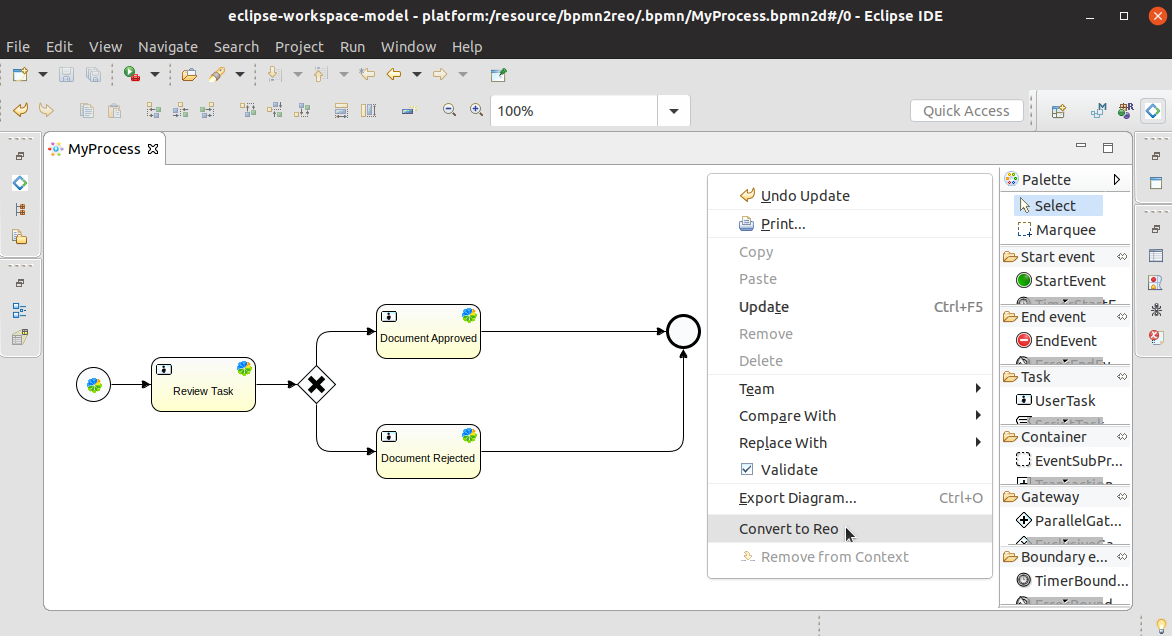
\includegraphics[width=.9\textwidth]{img/ectlast}
\caption{The BPMN to Reo converter menu in ECT}
\label{fig:ectscreen}
\end{figure}


\begin{figure}[!t]
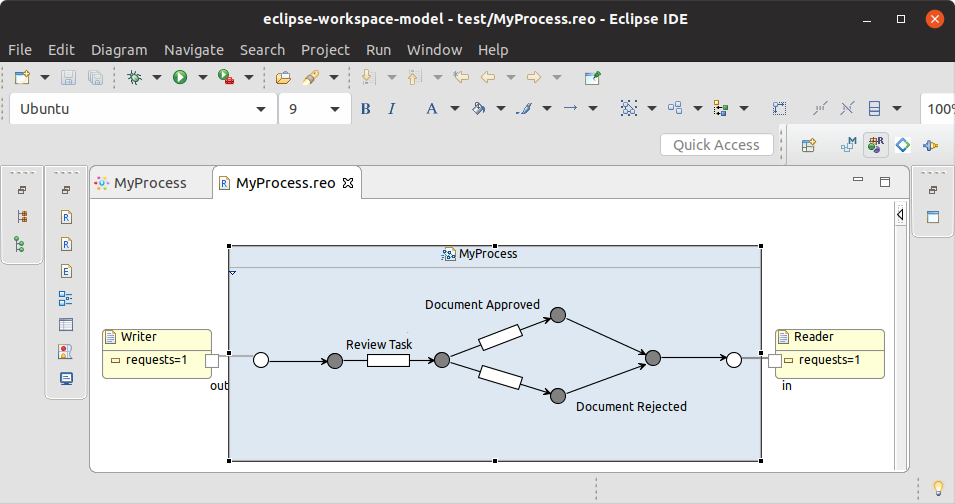
\includegraphics[width=.9\textwidth]{img/reofake}
\caption{The mapping of Figure \ref{fig:ectscreen}}
\label{fig:ectscreen2}
\end{figure}

\item We provide an extensible constraint-based approach to unify various semantic models of Reo networks. We represent a problem of computing semantics for a complex Reo network by encoding semantics of individual channels as constraints and solving the corresponding constraint satisfaction problem.
%
%
%Our framework is a place for different formal semantics of Reo to coexist and to complement each other. Our framework is based on constraint satisfaction problem,
%This is a generic and flexible way for encoding new behavioral models in the our framework. 
 This approach bridges the expressiveness gap and inconsistency among different Reo semantics. In addition, using a constraint-based approach replaces direct implementations of algorithms for calculating different Reo formal semantics.
%  off-the-shelf constraint solvers instead of direct implementation of custom algorithms to obtain semantics of Reo models. To mitigate inconsistency between behaviors described by different semantic models of Reo, we enforce the constraints of several formal semantics, which results into the behaviors that comply with all the semantics on the hand.

\item We extend our constraint-based framework to support the priority-aware behavior of Reo connectors. Priority is an important concept in modeling transactions. Our work makes it  more straight-forward and less complicated to obtain Constraint Automata with Priority (CAP) formal semantics for Reo. %, which also takes data and context-sensitivity into consideration.
	Our framework is the only existing approach that integrates various behavioral aspects of a Reo network (e.g. data-dependency, context-sensitivity, priority-awareness) under one umbrella.
 
%\item We have integrated our work into Ex
%\item Test  present a testing framework which support data-aware networks Chapter
\end{itemize}

\section{Outline}
The rest of this dissertation is organized as follows:

\begin{itemize}
\item In Chapter \ref{ch:bpmn}, we introduce BPMN 2 modeling elements and introduce an example of BPMN with problems. 

\item Chapter \ref{ch:reo} provides an overview of the Reo coordination language. There, we describe the behavior of Reo primitives in an informal style.

\item Chapter \ref{ch:formsem} overviews several formal semantics proposed for describing behavior of a Reo connector. The definitions of the semantics that are relevant to this work are given in details.

\item Chapter \ref{ch:mapping} describes our rule-based model-driven approach in transforming BPMN models to Reo connectors. %~\cite{bpmn}
%ing Notation (BPMN),  Business Process Execution Language (BPEL)~\cite{bpel} and the most common Unified Modeling Language (UML) 2.0~\cite{uml} dynamic models: Activity diagrams and Sequence diagrams. We have also developed tools for automatic transformation of these models into Reo~\cite{behnaz}. This enables the use of Reo analysis methods and tools on the coordination protocols that originally were not expressed in Reo. 
The transformation handles advanced BPMN elements, namely, transaction and compensation. 

An obstacle in computing execution semantics of some BPMN models with high-level elements such as transaction is that their behavior is too complicated and elaborated to directly be mapped to constructions of a language used for verification. To tackle this issue, we suggest a refinement procedure to substitute such high-level constructs with a set of simpler elements that together deliver the same functionality. %The  yet each of them is  easier to be 
This chapter is partially based on \cite{behnaz}.
 
\item In Chapter \ref{chapterCASM}, we introduce our constraint-based framework to capture the formal semantics of Reo networks, given by two different formal semantics namely, Constraint Automata with State Memory (CASM) and Connector Coloring (CC) \cite{coloring}. CASM is an extension of Constraint Automata (CA), which is one of the most popular semantics for Reo. We favor using CASM over CA, which is a simpler semantics, because CASM provides a mechanism to model the state values. This helps in treating the states symbolically. Therefore, unlike CA every data-item entering a buffer does not lead to a new state. %, which leads to a more compact representation of the automata.

To capture context sensitivity, a behavioral aspect that CA and some of its extensions miss, we use CC, which models context sensitivity in a Reo connector using graph coloring techniques.
%CA that due to its state abstraction and data-awareness, is suitable  as a more compact semantic model for Reo in model checking. In this chapter, 

We present a tool to generate CASMs from Reo networks in a compositional manner, where the part of behavior that is not compliant with CC is ruled out. 
% A shortcoming of earlier work stems from its lack of support for data-dependent behavior. We overcome this shortcoming in the work we present in this chapter. Our tool is a necessary step for providing fully automated model checking for data-aware and context-sensitive composition of services coordinated by Reo.

We employ highly optimized off-the-shelf constraint solvers instead of straight-forward custom algorithms for computing the semantics \cite{behconstraint}. We provide formal arguments to show the correctness of our approach. Then, we present an evaluation on the performance of our framework through a case study.
%increasing performance using constraint satisfaction techniques; and
%We explain each of these contributions in more detail below. Throughout
%this thesis we support our statements both in theory and in practice. We give formal
%arguments that show the correctness of our approach with respect to existing
%models, and present tools and benchmarks that confirm our claims.
%Decoupled execution and lightweight reconfiguration
%In this thesis we present the Dreams framework, a distributed framework for compositional
%
%We extends ideas behind Jose's constraint-based runtime engine for Reo to provide automated tools for %efficient??
%calculating the behavior of Reo networks

\item In Chapter \ref{ch:prio}, we extend our framework to support priority and its propagation through a Reo connector. We propose a constraint-based solution to replace the custom algorithm to calculate the priority-aware behavior of a Reo connector \cite{fsen19}. We first introduce a binary model of the priority and show how it can be encoded in our constraint-based framework, then we extend this solution to numeric priorities. We show the application of our model in a case study.
 %TODO refer to 
%We also overview the Extensible Coordination Tools \cite{ect} and present our contribution to this .

\item Chapter \ref{ch:concl} concludes this thesis and outlines future research directions. 
\end{itemize}

%This work is partially funded by the COMPAS \cite{compasproj}.% - Compliance-driven Models, Languages, and Architectures for Services (EU Framework 7 STREP project, Call 1, Theme ICT 1.1.2 Software and Services).% - Coordinator
%In this dissertation, we address the following research problems:
%\textbf{Problem 1: } 
%Existing tools for detecting behavioral errors, e.g., model checkers and verifiers do not work directly on BPMN models. Therefore, a majority of work aiming at analyzing BPMN maps them to other models with formal execution semantics. %Such model transformation enables model analysis on business processes.
%Various formalisms such as process algebra and Petri nets have been used for this purpose. However, when BPMN models are mapped to a process algebra notation, their initial structures is not preserved. This makes it difficult to point the elements back to their origin. In contrast, using Petri nets the initial structure is preserved. There are many model checker and simulator tools for Petri nets, but each tool performs different classes of analysis and some only can deal with a subset of Petri nets  \cite{RPU+07}.
%
%
%are well-suited for modeling, analyzing and describing concurrent systems
%with a complex process flow. There are many Petri net-based tools like Yasper [9],
%Woflan [19], INA [16], LoLA [17] and CPN Tools [14] that can be used for model
%checking and simulation. Different tools perform different types of analysis and some
%tools are limited to a subset of Petri nets that can be analyzed. Therefore, it is valuable
%to be able to use more tools. The range of analysis possibilities is extended by translating
%Petri nets to mCRL2, a process algebraic formalism. This enables automatic verification
%by the mCRL2 . 
%
%\textbf{Problem 2: } 
%We propose using Reo ~\cite{Arb04:mscs}, a channel-based language for exogenous coordination of software components and services, to model and analyze business processes. % due to its certain advantages:
%Kokash et al. in  \cite{bpmn2reo} \cite{KA09} have demonstrated the suitability of Reo to model behavioral patterns described by business process models. Based on these efforts, we have developed tools for automatic transformation of business process models into Reo~\cite{behnaz}. %This enables the use of Reo analysis methods and tools on the coordination protocols that originally were not expressed in Reo.
%Similar to Petri net, 
%Reo has graphical syntax and exact mathematical definitions of its execution semantics.  It 
% defines a form of coordination in terms of synchronizing, buffering, retaining data, etc., along with constraining its input and output data items. Reo allows hierarchical modeling where arbitrarily complex models can be formed out of simpler ones.  The semantics of Reo is compositional. This means that complex networks can be built by connecting simpler networks. 
%%This means that one can construct complex circuits by reusing simpler circuits. To be more explicit, two circuits can be glued together on their boundary nodes to form a new joint circuit. Unlike many other models of concurrency (e.g., pi-calculus \cite{sangiorgi2001the}), synchrony is preserved under composition. This means that if we compose a circuit with synchronous flow between nodes A and B with another circuit with synchronous flow between nodes B and C, the joint circuit has synchronous flow between nodes A and C. In other words, the composition of two synchronous circuits yields a synchronous circuit.
%\item Reo provides synchronous and asynchronous channels and supports propagation of synchrony. While synchronous communication in Petri nets are problematic and non-compositional. 
 %Reo better fits the paradigm of service-oriented computing, which in the past few years has become the common trend in Web system development. 
%The building blocks of a Reo model are \emph{channel}s. Each channel in 
%Similar to Petri nets related approaches, converting business processes to Reo has the advantage of preserving the structure of the original model. This is in contrast with other aforementioned formalisms such as process algebra. 
%
%Our proposed mapping of business models into Reo is implemented in a model based paradigm using Atlas Transformation Language (ATL) \cite{atl}, which is a high level rule-based  language dedicated to model transformation. Using ATL has enabled  us to benefit  from the power of separation of concerns and focus only on the required mapping rules, rather than matching patterns on the source models and execution of the rules.   %Model-To-Model Transformation with ATL | © 2008 by INRIA, Obeo; made available under the EPL v1.0
%
% Once a business model is transformed to a Reo network, its behavior can be formally studied using various programs within the Extensible Coordination Tools (ECT) \cite{ect},
% a set of Eclipse plug-ins that constitute an integrated development environment for   the Reo coordination language.  ECT contains tools for the design \cite{ect}, animation \cite{Krause11a} \cite{Krause201123}, simulation  \cite{oscarmaster}, testing ~\cite{aichernig2009fault}, stochastic analysis \cite{prismyoungjoo}, verification~\cite{vereofy}~\cite{KKdV10areo}~\cite{Mousavi04-ReoTechRep}, execution~\cite{SFM-2015-ArbabJ} \cite{JoseThesis} \cite{Jongmans2012}  \cite{Jongmans2013} \cite{ect}, and model transformation ~\cite{behnaz} \cite{Krause201123}  \cite{TVM+08} for Reo networks. 
%
%%the model checker Vereofy~\cite{vereofy}, the converter and model checker based on mCRL2~\cite{natmcrl2jor} and the stochƒastic analyzer tool integrated with Prism~\cite{prismyoungjoo}. 
% In addition, ECT provides a mapping of Reo connectors to mCRL2 language, which enables application of mCRL2 tool-set ~\cite{natmcrl2jor} . % on the busniess processes.
%
%%tomata or process algebra specifications suitable for automated analysis, or animated with the ECT animation engine. Figure \ref{fig:anim} shows an animation view that allows designers to simulate process execution step by step prior to its implementation. Figure \ref{fig:mcrl2} depicts a snapshot of the ECT view with the process algebra specification of this model suitable for model checking with the mCRL2\footnote{http://www.mcrl2.org/} . 
%Reo analysis tools work based on formal semantics of Reo models. Several operational semantics have been proposed for Reo \cite{sung30semantics} in various styles, namely, I/O streams~\cite{Arbab04RCC}, automata~\cite{BaierCA} \cite{KC09} \cite{} \cite{priority} \cite{CASMPourvatan2012}, connector coloring~\cite{coloring}, and constraints~\cite{JoseThesis}. 
%%%%Modeling, Testing and Executing Reo Connectors with the Eclipse Coordination Tools refrasho dararam ya az teze jose ya az teze yjm
%???The automatic analysis tools integrated in ECT include the model checker Vereofy~\cite{vereofy}, the converter and model checker based on mCRL2~\cite{natmcrl2jor} and the stochastic analyzer tool integrated with Prism~\cite{prismyoungjoo}. Related to the field of our interest, formal testing and test generation, Aichering et al.~\cite{aichernig2009fault} implemented a testing tool for Reo based on the rewriting logic Maude. They remark that since in Reo not every input event leads to an output, testing theories for finite state machines do not suit for testing Reo. In our previous work~\cite{kokash2011input}, we have employed the input-output conformance (ioco) testing theory for model-based testing and test generation for coordination  protocols modeled in Reo. There, we use the automata based underlying semantics of Reo to translate connectors to their equivalent process algebra, from which we  generate their corresponding input-output labeled transitions systems to feed to the TorX~\cite{torx}testing 
%The most basic automata-based semantics of Reo is Constraint Automata (CA)~\cite{BaierCA}. An advantage of CA and its extensions 
%%\cite{KC09} \cite{} \cite{CASMPourvatan2012} \cite{priority}
% is their support for data-constraints that are part of the coordination primitives in Reo. This is in contrast with the connector coloring semantics (CC) that abstract data-flow and express the behavior of a connector in terms of existence or lack of data-flow. 
%Constraint Automata with State Memory (CASM) \cite{CASMPourvatan2012} is an extension of CA that due to its state abstraction and data-awareness, is suitable  as a more compact semantic model for Reo in model checking. 
% Several operational semantics exist for Reo in various paradigms. 
%Each of the Reo semantics focuses on some behavioral aspects of a network and differs from the rest in terms of expressiveness. This leads to gaps between behaviors described by these semantics, meaning that part of behavior described by one semantics may not be considered valid by another semantics.
%
%There are many different formal semantis for Reo, while each focuses on a few behavioral aspects and ignores the rest. For example, \emph{Connector Coloring} semantics is data-unaware. Most variations of \emph{Constraint Automata} do not take context-dependent behaviors into consideration. None of the mentioned semantics supports the notion of priority. 
%
%As a result of ignoring some of the behavioral aspects, formal semantics can describe invalid behaviors for a given Reo connector. 
%
%For instatext. %, which in this case is the fact that an empty \emph{FIFO}$_1$ channel will always accept the incoming data item. 
%
%As another example, Figure \ref{fig:intprb12} depicts a Reo network consisting of two sequentially connected \emph{filter} channels, whose conditions are negation of each other. A \emph{filter} channel reads the incoming data item and evaluates its condition upon it. If the condition holds, the channel writes the data item out. Otherwise, it loses the data. As the CA semantics of this network in Figure \ref{fig:intprb22} shows, the node $c$ cannot have any data flow. However,  the CC semantics of the network, which is presented in Figure \ref{fig:intprb32} describes the possibility of data flow through the node $c$. This is because CC semantics is not a data-aware semantics.
%
%\begin{figure}
%\centering
%\begin{sub figure}[b]{.7\linewidth}
%\centering
%\mesallossyfif
%\subcaption{A context-sensitive Reo network whose behavior cannot be described solely by Constraint Automata}
%\label{fig:intprb1}
%\end{sub figure}
%%\quad \quad \quad \quad \quad
%\begin{sub figure}[b]{.7\linewidth}
%\centering
%   \vspace{1cm}
%   \begin{tikzpicture}[node distance=2.8cm, bend angle=35,auto,baseline=(q.base)]
%     %\tikz{%TCA for the \emph{timer} channel with early expiration
%		\node[state] (q) {$\ $};
%		\node[state,right of=q, node distance=3cm] (p) {$\ $}; %{\parbox{1.25cm}{$\ $}};
%		\path[transition] (q) edge [bend left] node[above,pos=.6] {\parbox{2.2cm}{$\ \ \ \{a, b_1, b_2\},\\ d(a)=d(b_1) \wedge d(b_2)=d(c)$} } (p)  
%		                  (q) edge [loop left] node[left,pos=.4] {$\{a\}, true$} (q)
%		                  (p) edge [bend left] node[below,pos=.5] {$\{a, c\}$, true} (q)
%		                  (p) edge [loop right] node[right,pos=.4] {$\{a\}, true$} (p)
%		                  (p) edge [] node[above,pos=.5] {$\{c\}, true$} (q); {A}
%	      %}
%    \end{tikzpicture}
%    \subcaption{Constraint automaton of the given network}
%\label{fig:intprb2}
%\end{sub figure}
%%\quad \quad \quad \quad \quad
%\begin{sub figure}[b]{.7\linewidth}
%\centering
%   \vspace{1cm}
% %  \begin{tikzpicture}
% %\hspace{1cm}
%  $ \begin{array}{cccc} a & b_1 & b_2 &c \\ 
%  - & - & - & \triangleright \\
%      \triangleright & \triangleright & \triangleright & \triangleright\\
%       \end{array}$ 
%  %  \end{tikzpicture}  
%  \vspace{.5cm}
%    \subcaption{Connector coloring semantics of the given network}
%\label{fig:intprb3}
%\end{sub figure}
%\caption{Example of a Reo network whose semantics cannot be solely expressed using Constraint Automata}
%\label{fig:formalsemprbs}
%\end{figure}
%
%\begin{figure}
%\centering
%\begin{sub figure}[b]{.7\linewidth}
%\centering
%\mesaldofilter
%\subcaption{A data-aware Reo network whose behavior cannot be described solely by Connector Coloring}
%\label{fig:intprb12}
%\end{sub figure}
%%\quad \quad \quad \quad \quad
%\begin{sub figure}[b]{.7\linewidth}
%\centering
%   \begin{tikzpicture}[node distance=2.8cm, bend angle=35,auto,baseline=(q.base)]
%     %\tikz{%TCA for the \emph{timer} channel with early expiration
%		\node[state] (q) {$q$};
%	%	\node[state,right of=q, node distance=3cm] (p) {\parbox{1.25cm}{$\ \ p(d)\\x<=t$}};
%		\path[transition] %(q) edge [bend left] node[above,pos=.6] {\parbox{2cm}{$\{a\}, x:=0,\\\ \ \ d:=\hat{a}$} } (p)  
%		              %    (p) edge [bend left] node[below,pos=.4] {\parbox{2.cm}{$\{b\}, x<t, \\ \hat{b}=d$} } (q)
%		                  (q) edge [loop right] node[right,pos=.3] {\parbox{2.5cm}{$\{a, b_1, b_2\}, \\ d(a) =d(b_1) \wedge  \\ d(b_1)=d(b_2) \wedge \\ p(a) \wedge p(b_1)$} } (q)
%		                  (q) edge [loop left] node[left,pos=.3] {\parbox{1.cm}{$\{a\}, \\ p(a)$} } (q)
%		                  (q) edge [loop above] node[above,pos=.3] {\parbox{1.cm}{$\emptyset, true$} } (q)
%		               %   (p) edge [] node[above,pos=.3] {\parbox{1.5cm}{$\emptyset,\ x=t$} } (q)
%		               ; {A}
%	      %}
%    \end{tikzpicture}
%    \subcaption{Constraint automaton of the given network}
%\label{fig:intprb22}
%\end{sub figure}
%%\quad \quad \quad \quad \quad
%\begin{sub figure}[b]{.7\linewidth}
%\centering
%   \vspace{1cm}
%  % \begin{tikzpicture}
%  $ \begin{array}{cccc} a & b_1 & b_2 & c \\
%   - & - & - & - \\
%    - & \triangleright & \triangleleft & \triangleleft \\
%  - & - & - & \triangleright \\
%  \triangleleft & \triangleleft & \triangleleft &\triangleleft \\
%   \end{array}$ 
%%    \end{tikzpicture}  
%%\vspace{1.5cm}
%  \vspace{.5cm}
%    \subcaption{Connector coloring semantics of the given network}
%\label{fig:intprb32}
%\end{sub figure}
%\caption{Example of a Reo network whose semantics cannot be solely expressed using Connector Coloring}
%\label{fig:formalsemprbs2}
%\end{figure}
%\textbf{Problem 3: } 
%Moreover, Reo is extensible, this means that new constructs can be introduced for modeling new behavioral aspects, such as priority.
%Moreover,
% Reo is an extensible language that is open for user-defined channels with new behaviors. However, since Reo formal semantics are segregated, there is no existing approach to incorporate new behavioral aspects into these semantics. Therefore, adding any new behavioral aspects requires defining new semantics. %We argue that lack of an extensible approach in modeling behavior of Reo connectors is the main reason behind abundance of Reo formal semantics. In contrast, our framework is generic and extensible. New behavioral aspects can be introduced to the framework by encoding them in terms of constraint.  % considered%It provides support for new behaviors by accepting the providing a unified approach of 
%As a matter of fact, we have extended this framework to include one of the least studied subject in Reo is priority. The notion of priority is necessary for modeling behaviors such as transaction and exception handling, where the data flow representing the error or exception should interrupt the normal flow. 
%\textbf{Problem 4: } 
%The notion of priority is necessary for modeling behaviors such as transaction and exception handling, where the data flow representing the error or exception should interrupt the normal flow. 
%A formal semantics to model priority in Reo, named Constraint Automata with Priority (CAP), has been proposed in \cite{priority}. CAP provides means to model propagation and stopping the propagation of priority. Despite its comprehensive approach in modeling priority, the proposed semantics is computationally expensive to be directly implemented. Similar to the other Reo formal semantics, CAP abstracts from important behavioral aspects such as context-sensitivity. % and time-awareness.
%
%In this thesis, we present a constraint-based framework to formulate priority and the propagation of priority in a Reo connector. %Our approach takes into account data, time, and context-sensitivity. We show the power of constraint satisfaction theory in modeling the behavior of Reo connectors.
%Several operational semantics have been proposed for Reo i.e \cite{sung30semantics} with various styles of I/O streams~\cite{Arbab04RCC}, automata, coloring~\cite{coloring} and constraints~\cite{JoseThesis}. The most basic automata-based semantics of Reo is Constraint Automata (CA)~\cite{BaierCA}. An advantage of CA and its extensions is their support for data-constraints that are part of the coordination primitives in Reo. This is in contrast with the coloring semantics that abstracts data-flow and expresses the behavior of a connector only in terms of existence or lack of data-flow.  
%In our recent work~\cite{KKV10}, we introduced support for the unified control and data flow analysis of the Reo process models with abstract data types using the mCRL2 .
% Such kind of analysis is not available in the aforementioned Penets based toolkits. Together with this contribution, the conversion of process models to Reo offers an automated model-driven approach to verifiable development of business processes and service-based systems.
%Several extensions for CA have been proposed, among them, Constraint Automata with State Memory (CASM)~\cite{CASMPourvatan2009}, Action Constraint Automata (ACA) \cite{kokash2010semantic}, and Quantitative Intensional Automata (QIA)~\cite{qia}. Each of these semantics focuses on certain aspects of Reo and is used in the areas that need its special expressiveness. The Extensible Coordination  (ECT)~\cite{ect} is a framework that integrates several tools to analyze Reo networks. Among them is the Reo animation engine~\cite{ect}, which allows a visual validation of the protocol by generating animated simulation of the connector. Although animation is useful for giving insight about the behavior of networks, due to its manual nature and lack of support for data-dependent behavior, its application is limited to special cases. 
%
%???The automatic analysis tools integrated in ECT include the model checker Vereofy~\cite{vereofy}, the converter and model checker based on mCRL2~\cite{natmcrl2jor} and the stochastic analyzer tool integrated with Prism~\cite{prismyoungjoo}. Related to the field of our interest, formal testing and test generation, Aichering et al.~\cite{aichernig2009fault} implemented a testing tool for Reo based on the rewriting logic Maude. They remark that since in Reo not every input event leads to an output, testing theories for finite state machines do not suit for testing Reo. In our previous work~\cite{kokash2011input}, we have employed the input-output conformance (ioco) testing theory for model-based testing and test generation for coordination  protocols modeled in Reo. There, we use the automata based underlying semantics of Reo to translate connectors to their equivalent process algebra, from which we  generate their corresponding input-output labeled transitions systems to feed to the TorX~\cite{torx}testing 
%Similar to most formal verification approaches, a major problem while working with ECT is the state explosion. %The freedom that Reo provide in having multiple concurrent data-flows is one of the origin of the  along with the data domain non-determinism in behavior of some channels are some origins of the bug state space.
 %Avoiding the state space explosion is crucial while dealing with data-dependent channels especially if we are interested in working with infinite data-domains. A traditional remedy for this problem is abstraction. In this chapter, we show how using computer algebra systems, namely Reduce~\cite{reduce}, can improve the situation. 
 %?The high degree of concurrency in Reo models makes a big state st  Another problem that a user face while working with the current Reo based  is 
%
%Our work has similarities with the distributed execution engine for Reo proposed in  \cite{JoseThesis}. However, there are major differences between these approaches. The framework for the Reo execution engine only
%provide support for synchrony and context-sensitivity, while ours deals
%with priority and is data-aware. Another difference is that the engine is concerned with finding a next step synchronization solution that can be seen as a portion of the operational semantics of a Reo network, while our framework calculates the whole semantics.
%
%We use Reo coordination language to model and formally analyze workflows. In this paper, we propose a constraint-based approach to formalize a notion of priority  for Reo. % In our previous work, we have presented a constraint-based framework that unifies various formal semantics of Reo. In this paper, we extend our framework to support priority. 
%We introduce special channels to propagate and block priority flow in Reo process models, define their semantics as constraints, and model data propagation via network as constraint satisfaction problem. 
%
%In \cite{behconstraint}, the authors proposed to model the semantics of Reo as a constraint satisfaction problem (CSP). This approach consists of defining data flow in a Reo network in the form of mathematical expressions on data observed on Reo nodes. The main advantage of such representation is the possibility to use existing constraint solvers to infer the behavior of a  network given the semantics of its constituent parts: nodes, channels, sub-networks, or external components. %For a given data input, the same method can be used to simulate the execution of a process. 
